\documentclass[a4paper,11pt]{article}

% Standart.
\usepackage[T1]{fontenc}
\usepackage[utf8]{inputenc}
\usepackage{lmodern}
\usepackage[french]{babel}
\usepackage{eurosym}

% Page format.
\usepackage{geometry}
\geometry{top=2cm, bottom=2cm, left=1cm, right=1cm}

% Figures.
\usepackage{graphicx}
\graphicspath{{resources/}}
\usepackage{float}
\usepackage{array}
\usepackage{tikz}

% Math and chemistry.
\usepackage{chemist}
\usepackage{siunitx}
\usepackage{numprint}
\usepackage{amsmath}
\usepackage{amssymb}
\usepackage{stmaryrd}

% Links. Should be loaded last.
\usepackage{hyperref}
\hypersetup{colorlinks=true,
            linkcolor=blue,
            filecolor=magenta,
            urlcolor=cyan,
            citecolor=blue}


% Useful environment
\newenvironment*{dummyenvironment}{}{}

% Custom commands
\newcommand{\R}{\mathbb{R}}
\newcommand{\Z}{\mathbb{Z}}
\newcommand{\N}{\mathbb{N}}
\newcommand{\der}{\,\mathrm{d}}
\newcommand{\e}{\mathrm{e}}
\newcommand{\ti}{\cdot}

\title{Compression}
\author{Guillaume TOCHON}
\date{17 mars 2018}

\begin{document}

\maketitle
\tableofcontents

\section{Compression de données}

Site slides : \url{www.lrde.epita.fr/~gtochon/CODO/}

Compression + decompression

Sans compression de donnees, un film 720p d'une heure ferait presque 400Gio.

La naissance naïve de la compression de données remonte aux environ du code
morse.
Shannon est responsable des fondements mathématiques.

Autre acteurs:
  - Abraham Lempel
  - David Huffmann
  - Terry Welch

\

Le but de la compression est que lors de la decompression, ce soit le moins
visible possible par l'utilisateur.

\

\subsection{Sur la compressabilité}

\subsubsection{Entropie}

On va chercher a eliminer les redondances, et les gaspillages.
L'outil que l'on va utiliser est l'entropie.

Du point de vue de Shannon, plus un message est probable, moins il contient
d'informations.

\

Prenons un alphabet $\Sigma$ de $N$ symboles
$$ \Sigma = \{s_1,s_2, ..., s_N\} $$

Avec leurs probabilités d'occurrence respectives
$$ p_i = p(s_i) $$

Évidemment, on a
$$ \sum_{i = 1}^{N} p_i = 1$$

\

Soit $F$ un fichier composé de $N_F$ éléments de $ \Sigma $.

Statistiquement, $s_i$ est présent $p_i \times N_F$ fois.

On définit $q_i$ la quantité d'information totale d'un symbole:

$$ q(s_i) = -log_2(p_i) $$

On a donc $Q_{Tot}$ la quantité d'information propre totale de $s_i$ contenue
dans $F$:

$$ Q_{Tot}(s_i) = -N_F \cdot p_i \cdot \log_2(p_i)$$

On définit donc $Q_{Tot}(F)$ la quantité d'information contenue dans un fichier
$F$:

\begin{align*}
  Q_{Tot}(F) &= \sum_{i = 1}^{N_F}(Q_{Tot}(s_i) \\
             &= \sum_{i = 1}^{N_F} -N_F \ti p_i \ti \log_2(p_i) \\
             &= -N_F \sum_{i = 1}^{N_F}p_i \ti \log_2(p_i)
\end{align*}

Or ce $-N_F$ devant la somme pose problème:  \textbf{la quantité d'information
  dépend de la taille du fichier}.

Cela implique qu'un gros fichier ``probable'' contient moins d'information qu'un
petit fichier improbable.

\

On définit donc l'entropie $H$ ainsi:

$$ H = \frac{Q_{Tot}(F)}{N_F} = - \sum_{i = 1}^{N_F}p_i \ti \log_2(p_i)$$

\

On notera en outre $Q_{Tot}$ avec le symbole $Sh$. On a bien évidemment:

$$ H \equiv Sh $$

\

On remarquera que l'entropie $H$ est \textbf{indépendante} de la taille du
fichier.

$H$ ne dépend donc que de l'alphabet considéré $\Sigma$ et de la distribution
des symboles qui compose le fichier $F$.

\subsubsection{Probabilités}

Soit $X$ une variable aléatoire telle que:

$$ X = \{x_1, x_2 ..., x_n\}$$

Et

$$ p_i = P(X = x_i) $$

On a donc l'espérance de $X$:

$$ E(X) = \sum_{i = 1}^nx_i \ti p_i = \sum_{i = 1}^nx_i \ti P(X = x_i) $$

Et on a donc:

$$ E(\varphi(X)) = \sum_{i = 1}^n \varphi(x_i) P(X = X_i) $$

\

On a donc, pour l'entropie:

\begin{align*}
  H &= - \sum_{i = 1}^{N_F}p_i \ti \log_2(p_i) \\
    &= \sum_{i = 1}^{N_F} \underbrace{(- \log_2(p_i))}_{q_i} \ti p_i \\
    &= \sum_{i = 1}^{N_F} q_i \ti p_i \\
    &= E(q(s_i))
\end{align*}

\subsubsection{Application à l'informatique}

On considère donc:

\begin{align*}
  N_\Sigma &= \{0, 1\} \\
  p(0) &= p_0 = p \\
  p(1) &= p_1 = 1 - p \\
\end{align*}

On a alors:

\begin{align*}
  H &= -p \ti \log_2(p) - (1 - p) \log_2(1 - p) \\
    &= H(p)
\end{align*}

Par convention, on pose:

$$ H = - \sum_{i = 1}^{N_F}p_i \ti \log_2(p_i) $$

$$ p_i \ti \log_2(p_i) = 0 \text{\quad si \quad} p_i = 0 $$

\subsubsection{Cas de l'entropie nulle (À corriger avec le prof)}

$H(0) = H(1) = 0$

On a des fichiers complètement désordonnés:

$$ p = 0 \implies F = \{1111...1\} $$

$$ p = 1 \implies F = \{0000...0\} $$

Donc l'entropie est nulle.


\

Quand $p = \frac{1}{2}$, les symboles sont équiprobables, le fichier est
complètement désordonné, donc complètement aléatoire. Dans ce cas, l'entropie
est donc \textbf{maximale}.

\

Voir la figure \ref{entropy_prob}.

\begin{figure}[!h]
  \centering
  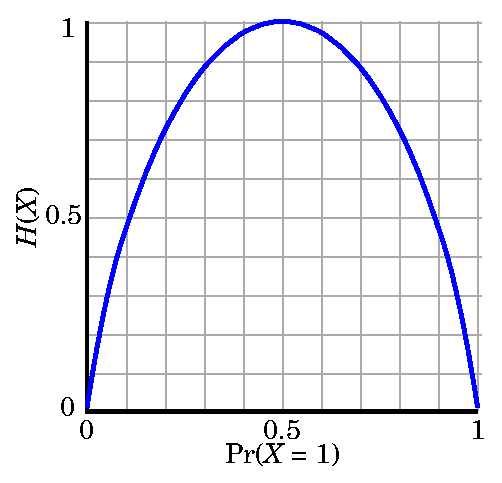
\includegraphics[width = 0.5 \textwidth]{Binary_entropy_plot.eps}
  \caption{Entropie en fonction de $P(X = 1)$}
  \label{entropy_prob}
\end{figure}

\

Attention! L'entropie ne voit pas les méta-symboles! Par exemple, ce fichier
est considéré comme parfaitement alétaoire:

$$ F = \{01010101\} $$

\subsubsection{Calcul de l'entropie}

Soit l'alphabet

$$ \Sigma = \{s_1, s_2, ..., s_N\} $$

De longeur:

$$ \forall n \in \N, \quad N_{\Sigma}= 2^n $$

Avec:

$$ \forall s_i \in \llbracket 1, N_{\Sigma} \rrbracket, \quad p(s_i) = p_i = \frac{1}{N_{\Sigma}} $$

On a donc:

\begin{align*}
  H &= - \sum_{i = 1}^{N_{\Sigma}}p_i \ti \log_2(p_i) \\
    &= - \sum_{i = 1}^{2^n} \frac{1}{2^n} \ti \underbrace{\log_2\left(\frac{1}{2^n} \right)}_{- n} \\
    &= \frac{1}{2^n} (-n) \underbrace{\sum_{i = 1}^{2^n} 1}_{2^n} \\
    &= n
\end{align*}

\subsubsection{Exercice}

De combien de bits a-t-on besoin pour encoder le fichier suivant?

$$ F = \{ACABBDDBAAABCAAA\} $$

Comptons le nombre d'occurrences de chacune des lettres de $\Sigma$ :

\begin{center}
  \begin{dummyenvironment}
    \left\begin{array}{ll}
           A: & 8 \\
           B: & 4 \\
           C: & 2 \\
           D: & 2 \\
         \end{array}
    \right\}
    \quad \text{Longeur: 16}
  \end{dummyenvironment}
\end{center}

\begin{enumerate}
\item Non compressé?

  C'est tout simplement, en notant $\Sigma$ l'alphabet utilisé pour encoder le
  fichier,

  \begin{align*}
    \text{Résultat} &= \text{Longeur} \times \text{Nombre de bits nécessaire
                      pour encoder } \Sigma \\
                    &= 16 \ti \log_2(n_{\Sigma}) \\
                    &= 16 \ti \log_2(4) \\
                    &= 32 \text{ bits}
  \end{align*}

\item Compressé?

  Calculons l'entropie du fichier:
  \begin{align*}
    H &= p_A \ti \log_2(p_A) + p_B \ti \log_2(p_B) + p_C \ti \log_2(p_C) + p_D \ti \log_2(p_D) \\
      &= \frac{1}{2} \ti \log_2\left(\frac{1}{2}\right) + \frac{1}{4} \ti \log_2\left(\frac{1}{4}\right) +
        \frac{1}{8} \ti \log_2\left(\frac{1}{8}\right) + \frac{1}{8} \ti \log_2\left(\frac{1}{8}\right) \\
      &= \frac{7}{4}
  \end{align*}

  Donc la longeur totale minimale du message est:

  \begin{align*}
    \text{Résultat} &= \text{Longeur} \times H \\
                    &= 16 \ti \frac{7}{4} \\
                    &= 28 \text{ bits}
  \end{align*}

\end{enumerate}












\section{Old}

$$
Q_{Tot}(S_{i}) = - N_{FP_{i}} Sh
$$ $$
Q_Tot(F) = Q_{Tot}(S_{1}) + Q_{Tot}(S_{2}) + ... + Q_{Tot}(S{N_{2}})
$$ $$
Q_{Tot}(S_{1}) = -N_{F}log_{2}(P_{i})
$$ $$
Q_{Tot}(S_{2}) = -N_{FP_{2}}log_{2}(P_{2})
$$ $$
Q_{Tot}(S{N_{2}}) = -N_{F}P_{N}log_{2}(P_{N})
$$ $$
Q_{Tot}(F) =  \sum -N_{FP_{i}}
= -N_{F} \sum P_{i}log_{2}(P_{i}) Sh
$$

Un gros fichier "probable" contient plus d'info qu'un petit fichier "improbable"
$
Q_{Tot} $ $\rightarrow$ Sh

$\rightarrow$ H $\rightarrow$ Sh/Symbole
$
H = - \sum P_{i}log_{2}(P_{i})$ $\rightarrow$ ne depend pas du fichier considere, mais uniquement
de la distribution de proba des symboles composant le fichier.



$X$ variable aleatoire de valeur $ \{ x_{1}, x_{2} ... x_{n} $
$\rightarrow$ $P_{i} = P(X = x) \sum P_{i} = 1$

$
E[X] = \sum_{i=1}^{N} x_{1} P(X = x_{i}) = \sum_{i = 1}^{N} x_{i} P_{i}
$ $
E[\phi (X)] = \sum_{i=1}^{N} \phi (x_{i})P_{i}
$ $
H= - \sum_{i= 1}^{N}P_{i}log_{2}P_{i} = \sum_{i = 1}^{N} (-log_{2}(Pi)) P_{i} = \sum_{i = 1}^{N}q_{S_{i} * P_{i}}
H = E[q(s_{i})]
$ $
\sum = {0,1} P(0) = P_{0} = P
             P(1) = P_{1} = 1 - P
$ $
H = -p log_{2}(p) - (1 - p) log_{2}(1 - p)
  = H(p)
$

---
Missing things
---



$\sum$ avec$ N $symboles $s_{i}, i = 1, .. N$
                                 $   (2^{n})$
$$
P(S_{i}) = \frac{1}{N_{\sum}} = \frac{1}{ 2^{n}}$$
$$
H = - \sum_{i = 1}^{N\sum} log_{2}(P_{i}) = - \sum_{i = 1}^{2^{n}}
  = -\sum_{i = 1}^{2^{n}} \frac{1}{2^{n}} log_{2} (\frac{1}{ 2_{n}}))
  = \frac{1}{ 2_{n}} * (-n) * \sum_{i = 1}^{2^{n}} * \sum_{i = 1}^{2^{n}} 1  
  = n2^{n}2^{-n} = n $$     (Sh/Symbole)


\end{document}
